\scanpage{47}
\mspage{19}

\deleted{\uline{privé} de $(\phi,\phi)$ (qui corresp. au drapeau $i,j$ lui $=$ \textendash{} si on ne l'excluait pas, on aurait une stratification de $\Sigma_{(i,j)}$ lui-$=$, non de son bord. Pour que $\Sigma_{ij}-\Sigma_i$ soit}
\margin{\deleted{\uline{(hyp. C.\unsure{$^{t}$|I})}}}
\deleted{lisse, il f. et s. donc que $j$ soit un successeur de $i$, et que $j$ soit \unsure{maximal} dans $I$}

élément (pour être fibré sur $\Sigma_i$) et $j$ comme dernier (pour être \unsure{contenus|contenu} ds $\Sigma_{ij}$) s'\unsure{ident} donc \inserted{$\simeq$} $\operatorname{Drap}(I_{i< <j})$. Il est vide ssi $j$ est un successeur de $i$, qui est donc la condition pour que $\Sigma_{ij}\unsure{-|\longrightarrow}\Sigma_i$ soit lisse.

Plus généralement, si $d\subsetneq d'$ est un segment initial, la fibration $\Sigma_{d'}\longrightarrow\Sigma_d$ est à fibres des variétés à bord, et le fibré des bords est stratifié cylindriquement par les $\Sigma_{d''}$ où $d''\supsetneq d'$ (pour que $\Sigma_{d''}\overset{\deleted{\unsure{\alpha}}}{\hookrightarrow}\Sigma_{d'}$) est tel que $d'$ soit cofinal dans $d''$ (pour que $\Sigma_{d''}\hookrightarrow\Sigma_{d'}$) et que $d$ soit segment initial dans $d''$ (pour que $\Sigma_{d''}\longrightarrow\Sigma_{d'}$ soit fibrant) i.e. \deleted{\unsure{si $d$ est le|si on est le}} \inserted{si $d'=(i_1-i_n)$}
$d=(i_1,-i_p)$, \deleted{\unsure{alors|donc} $d''$ \unsure{est de la forme}} d'où $d'=d\coprod d'_0$
\deleted{plus \unsure{grand élément} de $d_p$ et plus \unsure{grand élément}}
avec $d'_0=(i_{p+1},i_{p+2}\mathinner{\cdot-}i_n)$, alors les $d''$ correspondent aux

\noindent\begin{minipage}{\linewidth}
\leavevmode\rlap{\begin{tikzpicture}[overlay,x=1cm,y=1cm]
  \draw[line width=.35pt] (-.12,.16) -- (-.12,-1.03) .. controls (-.10,-1.17) and (.06,-1.20) .. (.27,-1.20) -- (8.15,-1.17) .. controls (8.52,-.98) and (8.19,-.68) .. (8.20,-.52);
  \draw[line width=.35pt] (2.05,-1.15) .. controls (3.51,-.61) and (5.85,.35) .. (5.69,-.16) .. controls (5.65,-.36) and (4.75,-.92) .. (5.03,-.83) .. controls (6.26,-.41) and (6.62,-.27) .. (7.16,-.38);
\end{tikzpicture}}
\deleted{\unsure{par $d'$} (\unsure{donc} $\alpha\leq\beta$), \unsure{ce sont} les drapeaux \unsure{ayant|où}}\\
\deleted{$\beta$ comme plus grand élément, et \unsure{formé d'indices}}\\
\deleted{\unsure{forme} $d\coprod d''_0$, où $d''_0\subset I_{\cdot>\alpha}$}
\end{minipage}

\inserted{\unsure{les|des} drapeaux \deleted{\unsure{finis}} $d''_0\subset I_{\cdot>i_p}$\unsure{)|,}} contenant \deleted{\unsure{$d_0$|les}} strictement $d'_0$ et tels que $d'_0$ soit cofinal dans $d''_0$, \deleted{\unsure{c'est donc un}} \inserted{l'un de ces $d''_0$, ou l'ens des $d''_0$, est en} corresp. biunivoque avec
\[
\operatorname{Drap}\bigl(I_{i_p<\cdot<i_{p+1}}\deleted{\unsure{\}|)}}\coprod I_{i_{p+1}<\cdot<i_{p+2}}\coprod\mathinner{-\,-\,\cdot}\coprod I_{i_{n-1}<\cdot<i_n}\bigr)
\]
\margin{46}
